\chapter{Results}
This chapter presents the findings of our study, organized into distinct experiments. Each experiment is designed to build upon the previous one, adding complexity. We begin with simple models to establish a baseline and progressively move towards more complex and realistic simulations. 

At this stage, we restate our guiding hypotheses:

\begin{itemize}
    \item \textbf{Hypothesis 1:} The use of PINNs will result in faster simulations of electric waves in  2D MRI-slice-based heart geometries compared to traditional methods.
    \item \textbf{Hypothesis 2:} PINNs can accurately simulate electrophysiological wave propagation in 2D MRI-slice-based heart geometries, including the incorporation of image informed scar tissue data.
    \item \textbf{Hypothesis 3:} A trained PINN can effectively extrapolate PDE parameters, such as conductivities, beyond the range of training data, providing accurate and reliable predictions.

\end{itemize}




\section{1D cable}
We begin this exploration by considering a $2\mathrm{cm}$ 1D cable domain. This experiment lays the foundation for the following experiments and allows us to compare our findings with existing literature \cite{EP-PINNs}. Additionally, we compare our PINN solution to a standard neural network (NN) trained with only the data without the physics loss components. The standard NN architecture and hyperparameters are the same as the PINNs in this experiment. 
\subsection{Data and Training 1D cable}
We generated synthetic data as outlined in \ref{data_structured}. The spatial domain was discretized with a step size of $\Delta x = 0.1$, and the time step used was $\Delta t = 0.005$. Different combinations of training sample sizes ($n=100,1000,10000$) and noise levels ($\sigma=0,0.01,0.1$) were used to create the datasets. 
For each combination, $10$ separate models were trained, generating $10$ RMSE values by computing the error across evaluation points consisting of the remaining data. The hyperparameters are outlined in Section \ref{architecture}.

The training loss convergence of a 1D model trained with \( n = 100 \) and \( \sigma = 0.1 \) is illustrated in Figure \ref{fig:loss_1D}. The plot displays the evolution of different components of the loss, \( \mathcal{L}_{PDE} \), \( \mathcal{L}_{ODE} \), \( \mathcal{L}_{BC} \), \( \mathcal{L}_{IC} \), and \( \mathcal{L}_{data} \), on a logarithmic scale. The graph shows a general decrease in the loss values, indicating successful training and convergence of the model. Notably, the \( \mathcal{L}_{ODE} \) and \( \mathcal{L}_{PDE} \) components demonstrate significant reduction, highlighting the model's ability to satisfy the underlying physical equations. The \( \mathcal{L}_{data} \) loss component also decreases consistently, reflecting accurate fitting to the provided data points. Overall, the training process results in well-balanced optimization across most loss components, except for the boundary condition component, which increases to begin with before converging.

\begin{figure}[H]
  \centering
  \includegraphics[width=\linewidth]{Figs/1D/loss_history_1D_100_01.pdf}
  \caption{Training loss convergence of 1D model trained with $n=100$ and $\sigma=0.1$. The plot shows the evolution of different components of the total loss on a logarithmic scale.}
  \label{fig:loss_1D}
\end{figure}

\subsection{Predictions: 1D cable}
Figure \ref{fig:pinn_vs_rk4} illustrates the comparison between the PINN prediction and the reference RK4 solution for the 1D cable model. Additonally, the figure shows the predicted solution from a standard neural network (NN) trained with only the data without the physics loss components. The state variable \( V \) is plotted as a function of time \( t \) at a randomly selected spatial location \( x \). The figure demonstrates that the PINN prediction closely follows the RK4 solution, indicating the effectiveness of the PINN in capturing the dynamics of the system. Even with a noise level of $\sigma = 0.1 $ (approximately $10\%$ of the maximum value of $V$) and a limited number of spatio-temporal points (\( n=100 \)), the PINN successfully approximates the reference solution with considerable accuracy with $\mathrm{RMSE}=0.07\mathrm{AU}$. In comparison, the standard NN achieves an RMSE of $0.15\mathrm{AU}$ shows tendencies to overfit the data by interpolating the training data rather than learning the underlying dynamics.

\begin{figure}[H]
  \centering
  \includegraphics[width=\textwidth]{Figs/1D/V_1D_PINN_NN_100.pdf}
  \caption{Comparison between the PINN prediction and the reference RK4. The blue line represents the PINN prediction, the orange line represents the RK4 solution, and the green crosses indicate the training data for the specific spatial location. The number of training points is \( n = 100 \) and the noise level is \( \sigma = 0.1 \).}
    \label{fig:pinn_vs_rk4}
\end{figure}
Figure \ref{fig:pinn_vs_rk4} illustrates the comparison between the PINN prediction, NN prediction, and the reference RK4 solution for the 1D cable model. The figure demonstrates that the PINN prediction again closely follows the RK4 solution. The PINN successfully approximates the reference solution with considerable accuracy with $\mathrm{RMSE}=0.02\mathrm{AU}$ when trained using $n=1000$ data points and a noise level with a standard deviation of $\sigma=0.1$. In comparison, the standard NN achieves an RMSE of $0.05\mathrm{AU}$ and shows less tendencies to overfit the data as in the previous case (Figure \ref{fig:pinn_vs_rk4}).
\begin{figure}[H]
  \centering
  \includegraphics[width=\textwidth]{Figs/1D/V_1D_PINN_NN_1000.pdf}
  \caption{Comparison between the PINN prediction and the reference RK4. The blue line represents the PINN prediction, the orange line represents the RK4 solution, and the green crosses indicate the training data for the specific spatial location. The number of training points is \( n = 1000 \) and the noise level with \( \sigma = 0.1 \).}
    \label{fig:pinn_vs_rk4_1k}
\end{figure}

\subsection{Evaluation 1D cable}
Figure \ref{fig:RMSE_1D} displays the RMSE values for different combinations of training sample sizes, $n$, and noise levels sampled from a normal distribution with standard deviation $\sigma$. The IQRs are larger for higher noise levels as well as for smaller training sample sizes, showing greater variability in the results. We see that as the number of training points increases, the addition of noise becomes less significant. Additionally, we see some outliers where the models have converged to a less optimal solution.
\begin{figure}[H]
  \centering
  \includegraphics[width=\textwidth]{Figs/1D/box_plot_1D_final.pdf}
  \caption{Box plot of RMSE values computed across evaluation points for different combinations of training sample sizes ($n=10^2,10^3,10^4$) and noise levels ($\sigma=0.0,0.01,0.1$). The blue colored boxes represent the IQR, indicating the middle $50\%$ of the computed RMSE. The orange lines within the boxes show the median values. The whiskers (thin blue lines) extend from the smallest to the largest values, excluding outliers (orange dots).}
  \label{fig:RMSE_1D}
\end{figure}

\section{2D structured geometry}
\subsection{Data and Training on a 2D Square}
Building on the 1D simulations, we now consider a $1\mathrm{cm}\times1\mathrm{cm}$ 2D structured grid domain. The spatial domain was discretized with a step size of $\Delta x = 0.1$, and the time step used was $\Delta t = 0.005$. As for the 1-D cable, different combinations of training sample sizes ($n=1000,10000,10000$) and noise levels ($\sigma=0,0.01,0.1$) were used to create the datasets. Due to the added complexity from the additional spatial dimension, the neural network inputs now include 2D spatial coordinates and time (x, y, t).

\begin{figure}[H]
  \centering
  \includegraphics[width=\linewidth]{Figs/1D/loss_history_2D_1000_01.pdf}
  \caption{Training loss convergence of 1D model trained with $n=100$ and $\sigma=0.1$. The plot shows the evolution of different components of the total loss on a logarithmic scale.}
  \label{fig:loss_2D}
\end{figure}
The training loss convergence of a 2D square model trained with \( n = 1000 \) and \( \sigma = 0.1 \) is illustrated in Figure \ref{fig:loss_2D}. The plot displays the evolution of different components of the loss, \( \mathcal{L}_{PDE} \), \( \mathcal{L}_{ODE} \), \( \mathcal{L}_{BC} \), \( \mathcal{L}_{IC} \), and \( \mathcal{L}_{data} \), on a logarithmic scale. The graph shows a general decrease in the loss values, indicating successful training and convergence of the model. Notably, the \( \mathcal{L}_{ODE} \) and \( \mathcal{L}_{PDE} \) components demonstrate significant reduction, but with larger fluctuation than seen in the 1D case (Figure \ref{fig:loss_1D}). The \( \mathcal{L}_{data} \) loss component decreases rapidly in the beginning of training, followed by a minimal, but steady decrease. 



\subsection{Predictions on a 2D Square}

Figure \ref{fig:2D_prediction} shows a comparison between the PINN prediction and the reference RK4 solution for the 2D structured grid model. The scalar field $V$ is depicted across the spatial domain at a randomly chosen time point. The PINN accurately captures planar wave dynamics with some deviations at the wave front and resting potential area ($0\mathrm{AU}$), even in the presence of noise with a standard deviation of about $10\%$ of the maximum value of $V$. 
\begin{figure}[H]
  \centering
  \includegraphics[width=\textwidth]{Figs/1D/2D_1000_0.1.png}
  \caption{Comparison of the state variable \( V \) between the RK4 reference solution and the PINN prediction in a square domain. The red crosses indicate the training data points for this specific time step. The number of training points is \( n = 1000 \) and the noise level is \( \sigma = 0.1 \).}
  \label{fig:2D_prediction}
\end{figure}

\subsection{Evaluation of results on a 2D Square}
Figure \ref{fig:RMSE_2D} displays the RMSE values for different combinations of sample sizes and noise levels, with RMSE computed across evaluation points. For each combination of \(n\) and \(\sigma\), 10 RMSE values are generated by training 10 separate models. Similarly to the 1D scenario, the interquartile ranges are larger for higher noise levels as well as for smaller training sample sizes, and as the number of training points increases, the addition of noise becomes less significant. Certain models in the 2D scenario display RMSE values that deviate significantly from the norm, both on the higher and lower ends.
%The results indicate that, for \(n=10^2\), the RMSE values are higher, particularly as the noise level (\(\sigma\)) increases. The interquartile ranges (IQR) are larger for higher noise levels, showing greater variability in the results. As the number of training points increases to \(n=10^3\) and \(n=10^4\), the RMSE values decrease significantly, demonstrating a trend toward more accurate predictions. The IQRs also become smaller, indicating more consistent performance across the 10 runs. Outliers are more prevalent in the smaller sample sizes and higher noise levels.
\begin{figure}[H]
  \centering
  \includegraphics[width=\textwidth]{Figs/1D/box_plot_2D_final.pdf}
  \caption{Box plot of RMSE values computed across evaluation points for different combinations of training sample sizes ($n=10^3,10^4,10^5$) and noise levels ($\sigma=0.0,0.01,0.1$). The blue colored boxes represent the IQR, indicating the middle $50\%$ of the computed RMSE values. The orange lines within the boxes show the median values. The whiskers (thin blue lines) extend from the smallest and largest values, excluding outliers (orange dots).}
  \label{fig:RMSE_2D}
\end{figure}

\section{MRI-based 2D geometry with isotropic conductivities}
Extending to more complex and anatomically accurate models, the third experiment involved an MRI-based geometry with isotropic conductivities. 


%
\subsection{Data and training for an MRI-based 2D geometry with isotropic conductivities}

We generate data from Finite Element Method (FEM) simulations based on an MRI-derived geometry consisting of $72434$ vertices as described in Section\ref{method_MRI}. The simulations are carried out using a time step of $20\mathrm{\mu s}$, output every $5\mathrm{ms}$ for a total of $211$ time steps. The simulation consists of a single heartbeat with a duration of $1050\mathrm{ms}$

\begin{table}[h]
  \centering
  \begin{tabular}{|c|c|}
    \hline
    Parameter & Value \\ \hline
    $g_{et}$ & 1 \\ \hline
    $g_{it}$ & 1 \\ \hline
    $g_{il}$ & 0.2 \\ \hline
    $g_{it}$ & 0.2 \\ \hline
  \end{tabular}
  \caption{Isotropic conductivities}
  \label{tab:Isotropic}
\end{table}

Time series data where then sampled at \(n_s\) spatial locations, each with \(n_t = 211\) timesteps, to mimic a clinical setup where measurements are sparse in terms of spatial resolution, although the temporal resolution is usually high. This approach was employed to investigate the effectiveness of PINNs in reproducing a detailed transmembrane potential map from these sparse measurements. Furthermore, we look into the variability of the models' performance across different combinations of number of training samples($n_s=20,100,1000$) and added noise ($\sigma=0,0.08,0.8$). In doing so, we train ten separate models for each combination.

%The data for the 2D geometry is sourced from Finite Element Method (FEM) . The spatial and temporal points for the training from both methods are presented in Table \ref{table:data_summary}.

%Table with spatial points and time steps from FEM&PINN
\begin{comment}
\begin{table}[h]
  \centering
  \caption{Comparison of the number of spatial points ($n_s$) and time steps ($n_t$) used in FEM and PINN simulations.}
  \begin{tabular}{|c|c|c|}
    \hline
     \textbf{Metric} & \textbf{FEM} & \textbf{PINN} \\ \hline
    $n_s$ & $72434$ & $7243$ \\ \hline
    $n_t$ & $241$ & $30$ \\ \hline
  \end{tabular}
  \label{table:data_summary}
\end{table}

\begin{table}[h]
  \centering
  \caption{Manually tuned hyperparameter settings for a 2D MRI-based geometry.}
  \begin{tabular}{|c|c|}
    \hline
    \textbf{Hyperparameter} & \textbf{Choice} \\ \hline
    Epochs data & 15000 \\ \hline
    Epochs total& 59000 \\ \hline
    Activation & tanh \\ \hline
    Layers & 6 \\ \hline
    Nodes & 128 \\ \hline
    Weight initialization & Glorot uniform \\ \hline
    $\eta$ & 0.008 \\ \hline
    
  \end{tabular}
    \label{table:2D_heart_hyper}
\end{table}

\begin{figure}[H]
  \centering
  \begin{subfigure}{.5\textwidth}
    \centering
    \includegraphics[width=\linewidth]{Figs/losses.pdf}
    \caption{A subfigure}
    \label{fig:sub1}
  \end{subfigure}%
  \begin{subfigure}{.5\textwidth}
    \centering
    \includegraphics[width=\linewidth]{Figs/losses_PDE_test_train.pdf}
    \caption{A subfigure}
    \label{fig:sub2}
  \end{subfigure}
  \caption{A figure with two subfigures}
  \label{fig:test}
\end{figure}
\end{comment}


%Show geometry
\subsection{Predictions for an MRI-based 2D geometry with isotropic conductivities}

Figure \ref{fig:2D_MRI_iso} displays the spatial distribution of the membrane potential (\(V_m\)) in a 2D MRI-based geometry at two different time points, 100 ms and 530 ms. The model was trained using $100$ randomly sampled spatial locations including the complete time series with $211$ timesteps. The relative $L^1$ error between the FEM and PINN results is provided, indicating an error of $0.02$ for both time points, while the relative $L^2$ error is $0.05$ and $0.04$ at $100 \mathrm{ms}$ and $530 \mathrm{ms}$ respectively. The errors computed accross the whole simulation were $RL^1=0.02$ and $RL^2=0.05$.
This indicates a very close match between the FEM and PINN solutions, and demonstrates the effectiveness of PINNs in handling complex geometrical structures derived from MRI data. In particular, this experiment shows that PINNs can reproduce the dynamics of electrophysiological wave propagation from sparse measurements and noisy measurements, critical in a clinical setting where data are often limited and have various sources of noise limiting their quality. However, some discrepancies at the wave-fronts can be observed at $t=100\mathrm{ms}$.
\begin{figure}[H]
  \centering
  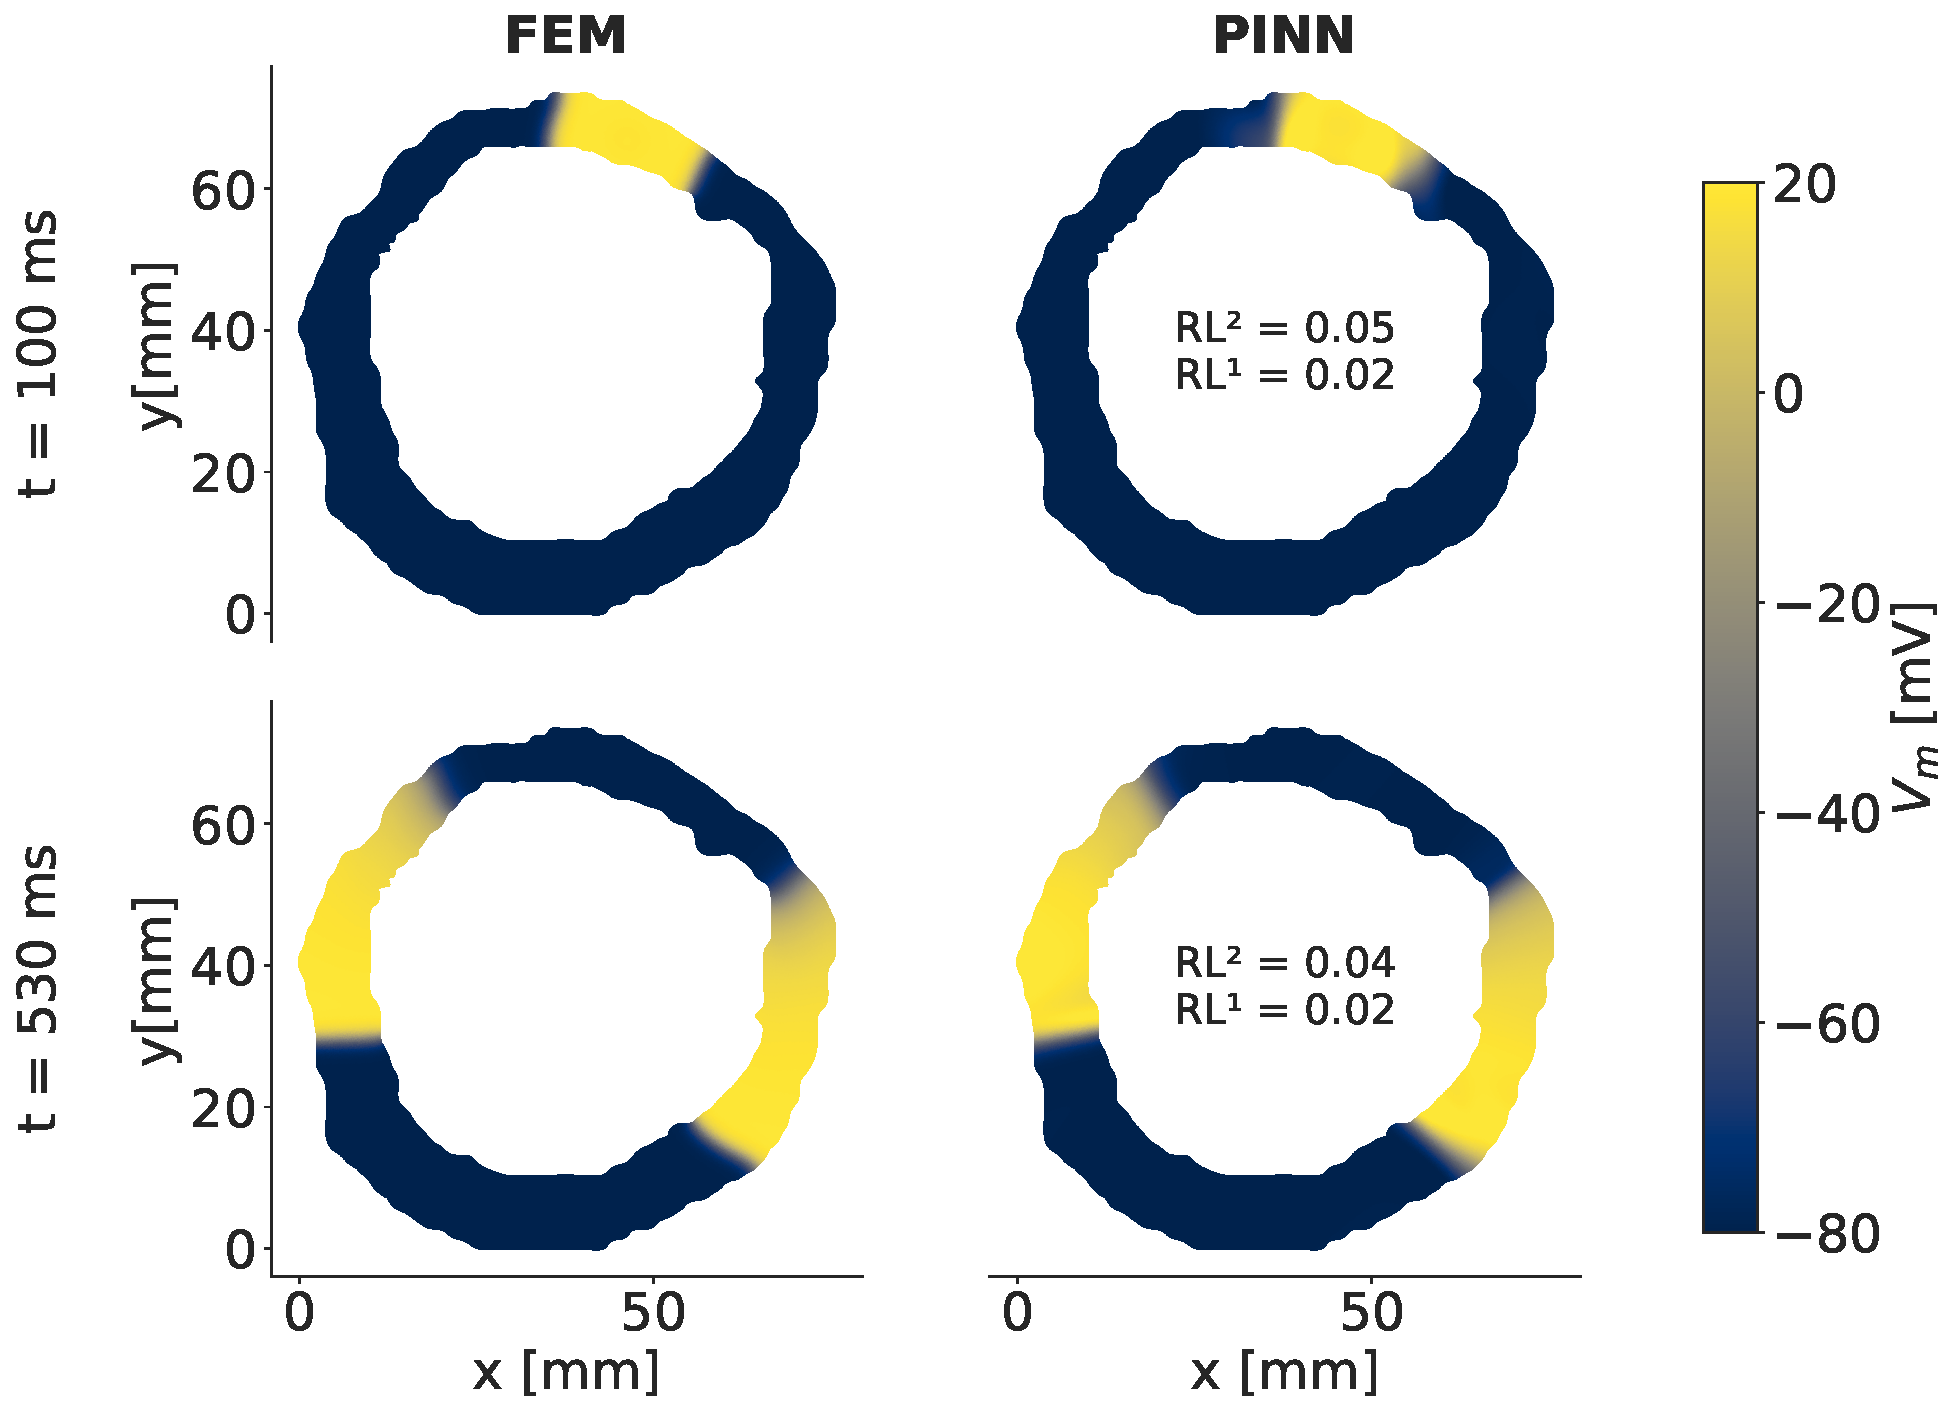
\includegraphics[width=0.9\linewidth]{Figs/Isotropic/subplots_RL2.pdf}
  \caption{Predictions with isotropic and homogeneous conductivities \( g_{il} = g_{it} = 0.2 \) S/m. The left column shows the results from the FEM at \( t = 100 \) ms and \( t = 530 \) ms, while the right column shows the predictions from the PINN at the same time points. The corresponding relative \( L^1 \) errors are computed for each timestep and are $0.02$ at both \( t = 100 \) ms and \( t = 530 \) ms. The number of spatial locations used in training is $n_s=100$ with noise level with $\sigma=8~\mathrm{mV}$.  }
  \label{fig:2D_MRI_iso}
\end{figure}





%Prediction within data timeframe: comparison og pred vs GT, Prediction time
%   
%Extrapolation: comparison og pred vs GT, Prediction time 
\subsection{Evaluation of an MRI-based 2D geometry with isotropic conductivities}
Figure \ref{fig:box_plot_MRI} displays the relative $L^1$ error computed across evaluation points for different combinations of sample sizes and noise levels.   As seen previously, the IQRs are larger for higher noise levels and a sparse training sample size, showing greater variability in the results. As the number of training points increases, the $RL^1$ values decrease and the addition of noise becomes less significant. The IQRs also become smaller, indicating more consistent performance across the 10 runs.
\begin{figure}[H]
  \centering
  \includegraphics[width=0.9\textwidth]{Figs/Isotropic/box_plot_iso.pdf}
  \caption{Box plot of the relative \( L_1 \) error of PINN predictions for the MRI-based model with isotropic and homogeneous conductivities. The x-axis labels indicate different training configurations, varying the number of spatial locations (\( n_s \)) and the standard deviation of noise (\( \sigma \)). }
  \label{fig:box_plot_MRI}
\end{figure}
\newpage
\section{MRI-based geometry with Anisotropic Conductivities}

In this experiment, we extend the MRI model to handle variable conductivity values as inputs, enbaling predictions with differing conductivities without retraining.


\subsection{Data and Training for an MRI-based geometry with Anisotropic Conductivities}

%\setlength{\textfloatsep}{0.1pt} % Adjust vertical space between floats
%\setlength{\intextsep}{1pt} % Adjust space above and below in-line floats
\begin{multicols}{2}
The data was generated from multiple FEM simulations with fixed extracellular conductivities (\(g_{el} = 1~\mathrm{S/m}\), \(g_{et} = 1~\mathrm{S/m}\)) and intracellular transverse conductivity (\(g_{it} = 1~\mathrm{S/m}\)), while varying intracellular longitudinal conductivity (\(g_{il}\)) from 0.5 to 1 in steps of 0.05. Conductive heterogeneities, representing scars, were introduced in the specified regions, marked in blue in Figure \ref{fig:scar}, with conductivities as shown in Table \ref{tab:scar_conductivities}. 
The model was trained with a subset of the datasets ($g_{il}=0.5,0.6,0.7,0.8,0.9$), from which we sample $N=10^6$ spatio-temporal points.

\begin{table}[H]
  \centering
  \begin{tabular}{|c|c|}
    \hline
    Parameter & Value \\ \hline
    $g_{il}$ & $0.0775~\mathrm{S/m}$ \\ \hline
    $g_{it}$ & $0.0143~\mathrm{S/m}$ \\ \hline
    $g_{el}$ & $0.2785~\mathrm{S/m}$ \\ \hline
    $g_{et}$ & $0.0512~\mathrm{S/m}$ \\ \hline
  \end{tabular}
  \caption{Scar conductivities.}
  \label{tab:scar_conductivities}
\end{table}


\begin{figure}[H]
    \centering
    \includegraphics[width=0.8\linewidth]{Figs/Anisotropic/scar_region.pdf}
    \caption{Heterogeneous conductivity map. Conductivities in the scar-region (blue) are fixed and shown in Table \ref{tab:scar_conductivities}. The grey area has conductivities with varying $g_{il}$.}
    \label{fig:scar}
\end{figure}



%\setlength{\textfloatsep}{20pt} % Adjust vertical space between floats
%\setlength{\intextsep}{10pt} % Adjust space above and below in-line floats

\end{multicols}
\newpage

Figure \ref{fig:loss_aniso} presents the convergence behavior of the loss function components during the training of an anisotropic and heterogeneous MRI-based model. The plot illustrates the evolution of different loss terms, namely $\mathcal{L}_{PDE}$, $\mathcal{L}_{ODE}$, $\mathcal{L}_{BC}$, $\mathcal{L}_{IC}$, and $\mathcal{L}_{data}$, over training steps on a logarithmic scale. 

We see all loss components decrease rapidly during the initial phase of training, and the loss being dominated by the data component.
\begin{figure}[H]
  \centering
  \includegraphics[width=\linewidth]{Figs/Anisotropic/loss_aniso.pdf}
  \caption{Anisotropic and heterogeneous MRI-based model training loss convergence during training on a logarithmic scale. The plot shows the evolution of different components of the total loss.}
  \label{fig:loss_aniso}
\end{figure}


\subsection{Predictions for an MRI-based geometry with Anisotropic Conductivities}



%INTERPOL
Figures \ref{fig:MRI_interpolation} and \ref{fig:MRI_extrapolation} present a comparison between the FEM reference solution and the PINN predictions when using conductivity inputs beyond the range of the training data. Both figures are produced using our best performing model in this experiment. In both figures, we see the PINN solution is able to accurately represent the transmembrane potential. Notably, we can see the wavefront slowing down when reaching the low-conduction zone(blue area in Figure \ref{fig:scar}) as the wave front curves around the scar area at $t=100 \mathrm{ms}$ in Figure \ref{fig:MRI_interpolation}, and at both $t=100 ms$ and $t=530 ms$ in Figure \ref{fig:MRI_extrapolation}. The deceleration of the wave is also evident, as the wavefront has propagated more to the right compared to the left between the two specified time points.
\begin{figure}[H]
  \centering
  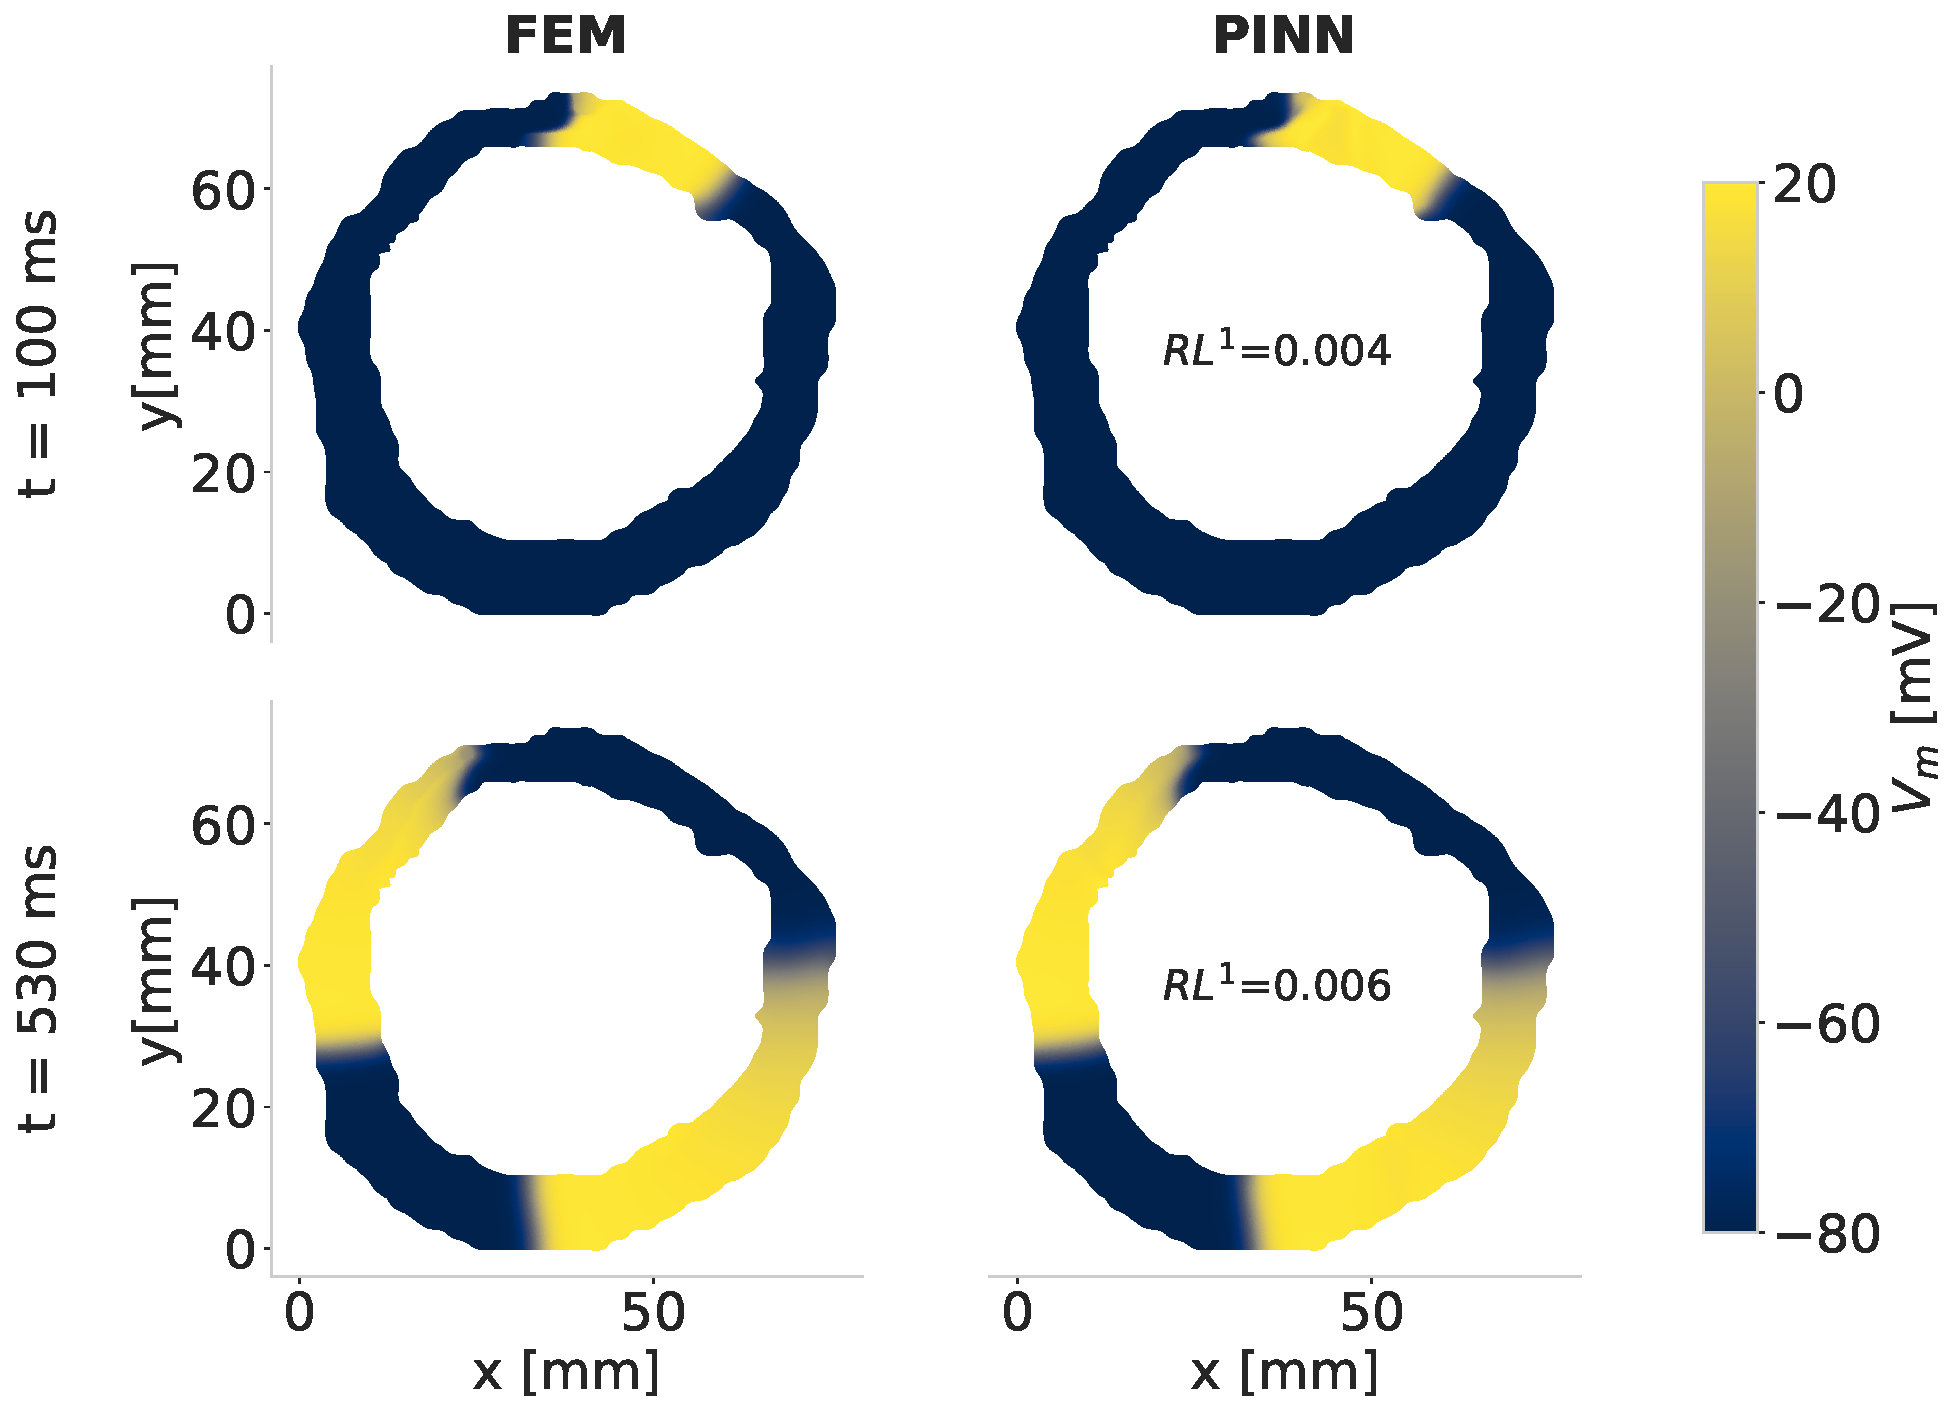
\includegraphics[width=0.8\linewidth]{Figs/Anisotropic/subplots_interpolation.pdf}
  \caption{Interpolated conductivity predictions of the best performing anisotropic model using \( g_{il} = 0.55 \), which is not included in the training data. The left column shows the results from the FEM at \( t = 100 \) ms and \( t = 530 \) ms, while the right column shows the predictions from the PINN at the same time points. The corresponding relative \( L_1 \) errors (\( RL_1 \)) are computed for each timestep and are 0.004 at \( t = 100 \) ms and 0.006 at \( t = 530 \) ms. The color bar indicates the membrane potential \( V_m \) in mV.}
  \label{fig:MRI_interpolation}
\end{figure}


\begin{figure}[H]
  \centering
  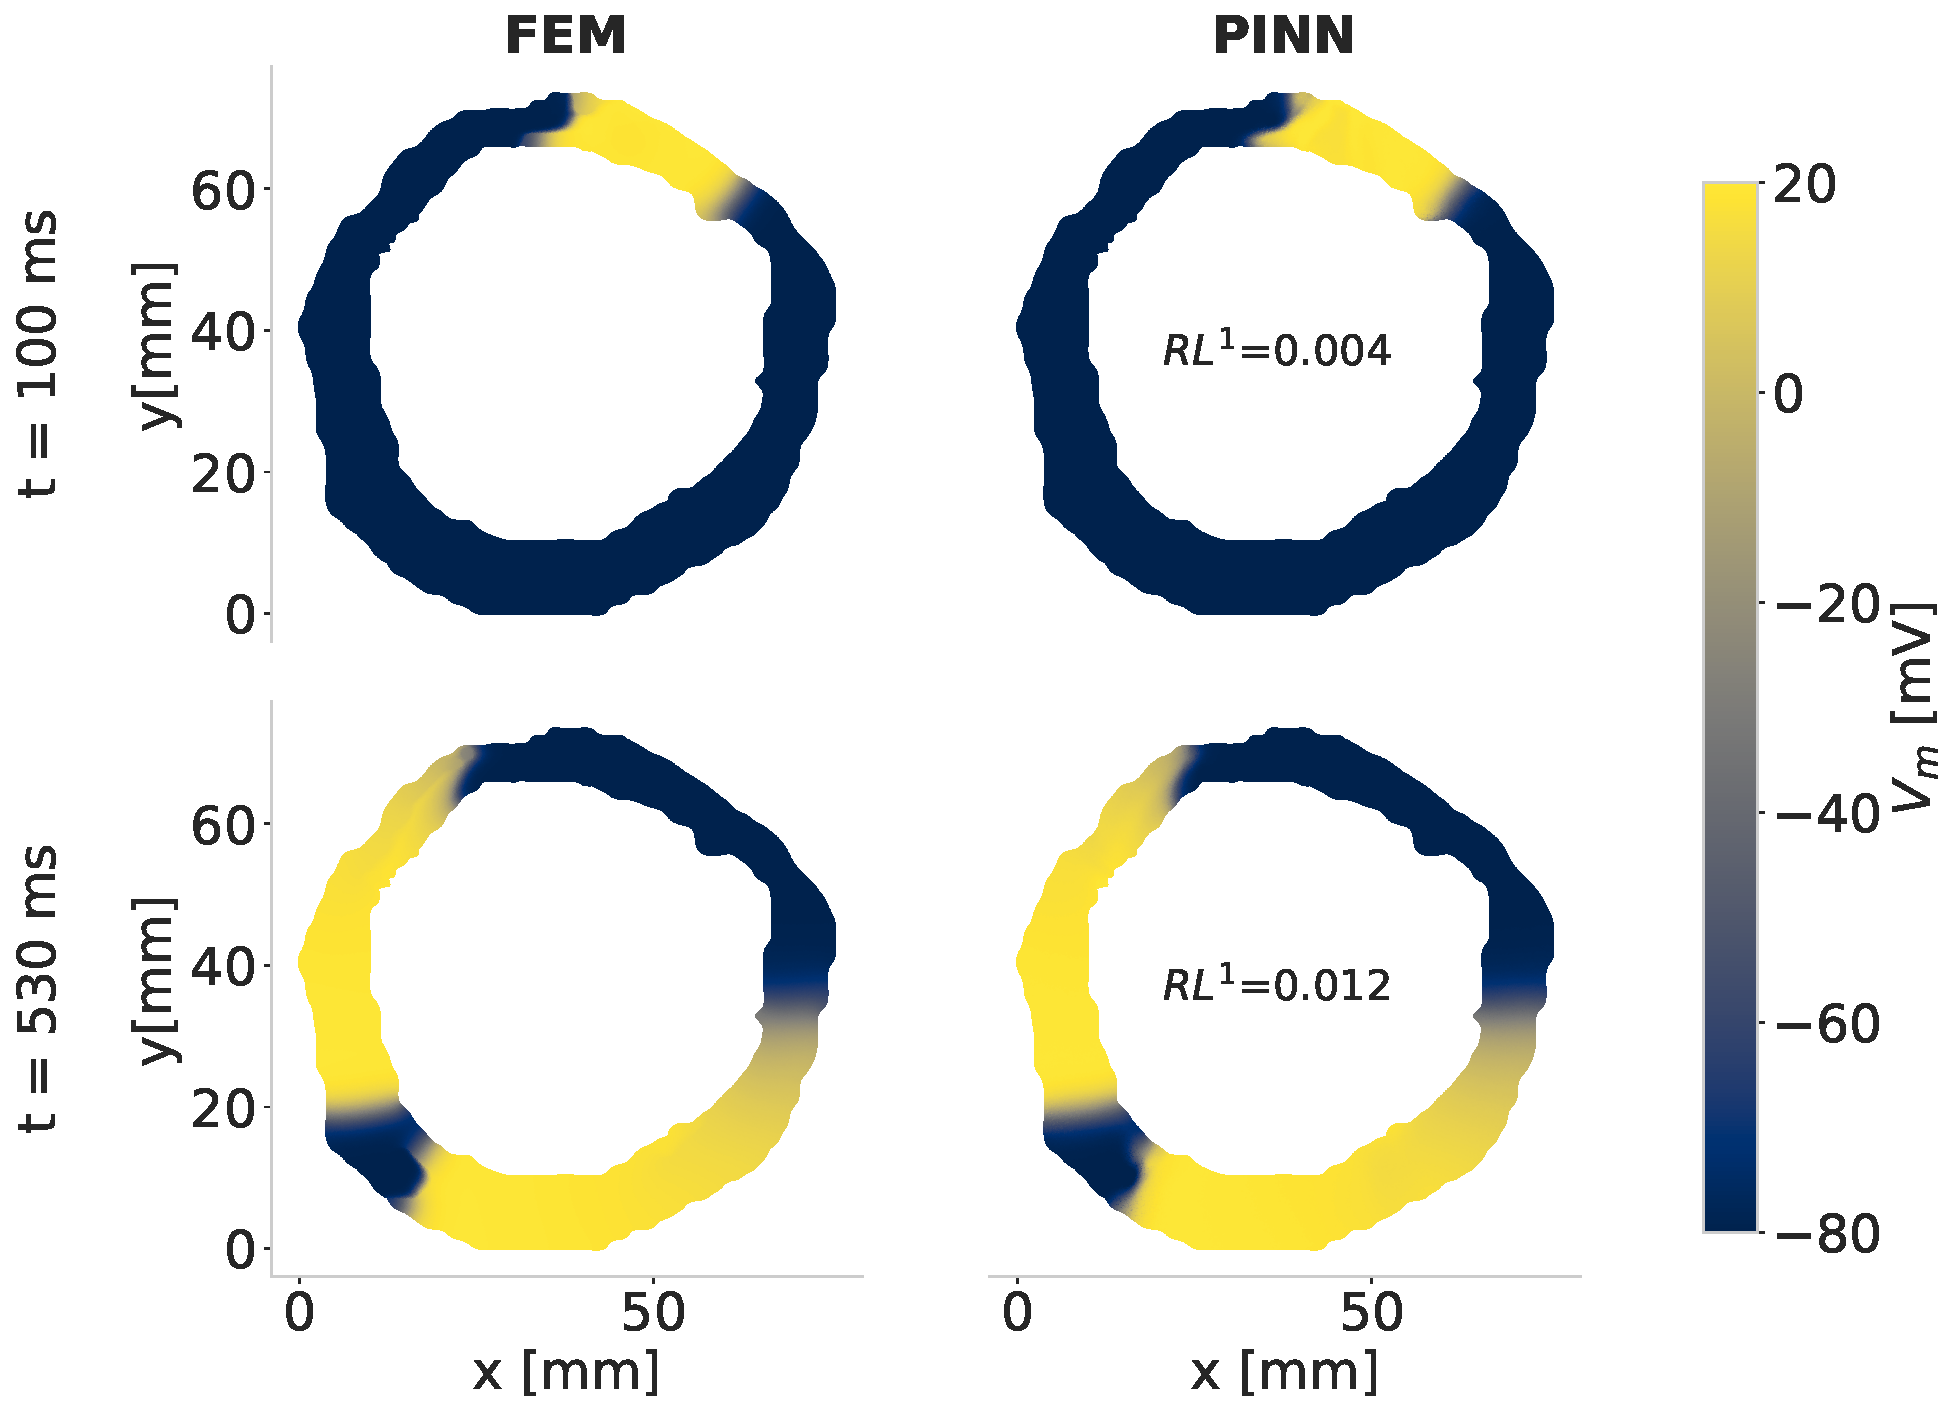
\includegraphics[width=0.8\linewidth]{Figs/Anisotropic/subplots_extrapolation.pdf}
  \caption{Extrapolated conductivity predictions of the best performing anisotropic model using \( g_{il} = 1 \), which is beyond the range of the training data. The left column shows the results from the FEM at \( t = 100 \) ms and \( t = 530 \) ms, while the right column shows the predictions from the PINN at the same time points. The corresponding relative \( L_1 \) errors (\( RL_1 \)) are computed for each timestep and are 0.004 at \( t = 100 \) ms and 0.012 at \( t = 530 \) ms. The color bar indicates the membrane potential \( V_m \) in mV.}
  \label{fig:MRI_extrapolation}
\end{figure}



\subsection{Model Evaluation of an MRI-based geometry with Anisotropic Conductivities}
%Figure \ref{fig:RL1_anisotropic} presents the relative L1 error computed from a model trained on a dataset generated by varying longitudinal intracellular conductivities (\(g_{il}\)). The results are highlighted for three scenarios: training data, interpolation, and extrapolation. The relative L1 error is observed to increase slightly during extrapolation beyond the training dataset's range, while it remains on par with the training data during interpolation.
%This figure highlights the model's performance and its ability to generalize across varying conductivity inputs.

Figure \ref{fig:RL1_anisotropic} shows the relative $L^1$ error computed with a model trained on a data set with varying longitudinal intracellular conductivities ($g_{il}$). The results are highlighted for three cases: training data, interpolation, and extrapolation. The relative $L^1$ error increases slightly during extrapolation beyond the range of the training data set, while it remains comparable to the training data during interpolation. This figure illustrates the model's performance and its capability to generalize across different conductivity inputs.


\begin{figure}[H]
  \centering
  \includegraphics[width=0.8\linewidth]{Figs/Anisotropic/L1_error_bar_plot.pdf}
  \caption{Relative $L^1$ error computed from the best performing MRI-based model with anisotropic and heterogeneous conductivities trained on a dataset generated by varying longitudinal intracellular conductivities $g_{il}$.}
  \label{fig:RL1_anisotropic}
\end{figure}


Figure \ref{fig:box_plot_MRI_aniso} illustrates the variability from training five separate models and shows the relative $L^1$ error ranges across training, interpolation, and extrapolation sets. Each round marker represents the mean relative $L^1$ error, and the whiskers indicate the standard deviation, providing a sense of the variability in the predictions.

The training data (green), interpolation data (blue), and extrapolation data (orange) show relatively consistent error ranges, with standard deviations reflecting the spread of the error values. The plot suggests that the model maintains stable performance across different conductivity values, with no significant increase in error for extrapolated data, highlighting the robustness of the model in handling varying input conditions. The consistent error across different sets demonstrates that the model can generalize well beyond the training data, which is crucial for practical applications involving variable conductivity values as discussed further in following Chapters.
%Each box represents the interquartile range (IQR), with whiskers extending from the smallest to the largest values, and the median and mean indicated by orange lines and pink markers, respectively. Training data (blue) and extrapolation data (green) display consistent error ranges, while interpolation data (orange) shows slightly lower variability. The plot suggests that the model maintains stable performance across different conductivity values, with no significant increase in error for extrapolated data, highlighting the robustness of the model in handling varying input conditions.
\begin{figure}[H]
  \centering
  \includegraphics[width=\textwidth]{Figs/Anisotropic/Mean_Errorbar_plot_aniso.pdf}
  \caption{Error bar plot of the relative \( L_1 \) error of PINN predictions for the MRI-based model with anisotropic and heterogeneous conductivities. The figure is generated by training $5$ separate models. The data set is generated by varying longitudinal intracellular conductivities $g_{il}$. The round markers indicate the mean and the whiskers indicate the standard deviation.  }
  \label{fig:box_plot_MRI_aniso}
\end{figure}
\newpage
The performance comparison in terms of inference time between the traditional FEM and the PINN approach is presented in Table \ref{tab:performance_comparison}. Simulation times using the FEM approach averaged $684 \pm 60$ seconds when running on a CPU (AMD Ryzen 4800H laptop CPU), indicating a significant computational effort required for a single simulation. 

\begin{wrapfigure}{r}{0.4\textwidth}
  \centering
  \begin{tabular}{| l | c | c |}
    \hline
     & FEM & PINN \\ \hline
    CPU & $684\pm60$ s & $3.62\pm0.09$ s \\ \hline
    GPU & - & $0.22\pm 0.01$ s \\ \hline
  \end{tabular}
  \caption{Comparison of FEM and MRI-based anisotropic PINN prediction inference time. The PINN time excludes the training time.}
  \label{tab:performance_comparison}
\end{wrapfigure}
In contrast, the PINN implementation demonstrated a markedly faster performance with an average CPU time of only $3.62 \pm 0.09$ seconds. Furthermore, when using a GPU (NVIDIA RTX3070 mobile), the PINN performance is enhanced even further, achieving an average computation time of just $0.22 \pm 0.01$ seconds per simulation, which is over $3000\times$ faster than FEM.
The training time is typically around $6-10\mathrm{h}$ when parallelizing training on five NVIDIA RTX 2080Ti. In comparison, generating the complete dataset with varying conductivities takes approximately $2\mathrm{h}$ with a time step of $20\mathrm{\mu s}$.
%In comparison, generating the complete dataset with varying conductivities takes approximately $8\mathrm{h}$ with a time step of $5\mathrm{\mu s}$.





